\lstdefinestyle{yaml}{
     basicstyle=\color{red}\footnotesize,
     rulecolor=\color{black},
     string=[s]{'}{'},
     stringstyle=\color{red},
     comment=[l]{:},
     commentstyle=\color{black},
     morecomment=[l]{-}
 }
 \lstset{numbers=left}
 
\chapter{Proof Of Concept} \label{ch:proofOfConcept}

This chapter explores the \gls{ac:poc} phase within the context of the thesis, aiming to validate the feasibility and efficacy of implementing \gls{ac:sdv} technologies. The main objective of this chapter is to translate theoretical concepts into concrete results, demonstrating the practical application of \gls{ac:sdv} in real-world situations. Through the \gls{ac:poc}, we aim to confirm the fundamental principles and features of \gls{ac:sdv}, including its potential impact on vehicle performance, user experience, and overall safety.

The multifaceted nature of \gls{ac:sdv} requires a structured approach to its implementation, taking into account factors such as standardized hardware, cloud integration, and \gls{ac:ota} updates. To achieve this, a \gls{ac:poc} was designed to address these components individually and holistically, ensuring a seamless integration that aligns with the envisioned paradigm shift in automotive manufacturing. Furthermore, this chapter aims to demonstrate the collaborative efforts with industry-leading technologies and platforms, highlighting the strategic partnerships forged with key players in the automotive and software development sectors. By aligning with renowned entities, the \gls{ac:poc} aims to leverage their expertise, technologies, and frameworks, thereby enhancing the robustness and scalability of the \gls{ac:sdv} ecosystem.

%Test and Validation are the concluding phases of this chapter, where the Proof of Concept is subjected to real-world scenarios. A demonstration involving a \textit{Raspberry Pi} (RPi) serves as a tangible validation of the implemented SDV functionalities. This section serves as the litmus test, affirming the seamless orchestration of SDV within the envisioned architecture.

The \gls{ac:poc} exploration utilizes the description of services and technologies provided by \gls{ac:aws} in \gls{ac:iot}, data management, and automotive industries, which are essential for the project's implementation.

Now, let's look at the components of the \gls{ac:poc} in detail through a high-level architectural representation of the previously introduced elements and a more detailed analysis of the code that compose them.

\section{Architectural design}
This section delves into the heart of the project implementation, starting with a high-level view of the various systems that make up its realization and transitioning to a visualization of the interactions between the various elements.

The study and analysis of the \gls{ac:sdv} case study revealed that three fundamental elements were essential to create a concrete example of \gls{ac:sdv} implementation:
\begin{itemize}
    \item \textbf{\gls{ac:tcu} simulator:} The \gls{ac:tcu} simulator is a system that replicates the basic functions of a telematic control unit (\gls{ac:tcu}). The system has the capability to send data packets and receive updates from a cloud server structure.
    \item \textbf{Cloud infrastructure:} The cloud infrastructure must be capable of managing both the data from the \gls{ac:tcu} and the update function.
    \item \textbf{Data viewer:}  The data viewer is a platform that enables the visualization of manipulated and processed data in a manner that clearly displays changes in data behavior resulting from variations in the data and updates to the \gls{ac:tcu}.
\end{itemize}

With these three elements, a practical implementation made it possible to achieve what should happen in an \gls{ac:sdv}: having a vehicle system capable of updating itself via \gls{ac:ota} updates. To support this implementation, it was necessary to use the services previously mentioned for creating the cloud infrastructure through the services made available by \gls{ac:aws}.

\subsection{TCU Simulator}
This project considers a \gls{ac:tcu} to be a hardware system capable of generating data from one or more subsystems of a potential vehicle, collecting it, and then preparing it for transmission outside the vehicle. To familiarize with this structure and to design the sample project, it was necessary to simulate a TCU in a way that was as close as possible to a real system, without having the availability of a real vehicle. Therefore, to simplify the concept, a \textit{Raspberry Pi} board was chosen as the \gls{ac:tcu} endpoint capable of generating telemetric data.

\begin{figure}[h]  % 'h' significa che la figura viene posizionata qui
    \centering
    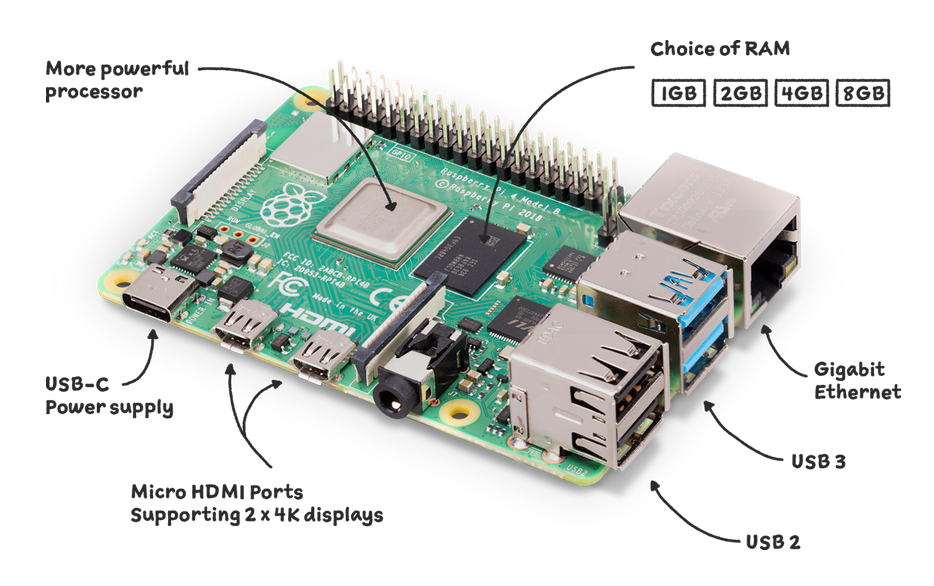
\includegraphics[width=0.8\textwidth]{images/raspberrypi.png}  % Sostituisci 'nome_immagine' con il nome del tuo file immagine e l'estensione
    \caption{Illustration of a \textit{Raspberry Pi} board with its periferics \cite{raspberrypi}}
    \label{fig:raspberrypi}
\end{figure}

As shown in the figure above \ref{fig:raspberrypi} a \textit{Raspberry Pi} is a board containing everything necessary to function as an independent system to which various peripherals can be attached, making it the ideal abstraction of a general-purpose \gls{ac:tcu} needed to implement the \gls{ac:sdv} case study.
Before working with the raspberry, it was necessary to implement the project on a virtual machine, which greatly facilitated the development and testing of the written code on a \gls{ac:pc} with a different operating system and architecture than the \textit{Raspberry Pi} board.

The simulator was thought to consist of four different software components, each with its own functionality, during its various stages of development:
\begin{itemize}
    \item A component is responsible for connecting to the cloud server to send telematics data;
    \item A component for establishing a connection to the cloud server in order to update the telematics unit;
    \item A component for generating telematics data;
    \item A component for recognizing and managing local unit updates.
\end{itemize}
An external script manages the startup of the simulation unit via command line using the four items. 

Analyzing these four elements in detail, the first element in chronological order was the component responsible for connecting the system to the cloud infrastructure via the \gls{ac:mqtt} protocol. This component required the presence of an active cloud-side IoT Core service, which, as we will discuss later, generates a certificate with an attached public and private key pair to ensure the device's identity. The consideration of the cloud infrastructure will be analyzed later when the cloud infrastructure is discussed.

In order to establish a connection to the cloud platform, the following code snippet from listing \ref{lst:MQTTConnection} is analyzed. The Python script launches and establishes a connection to the \textit{AWS IoT Core} server using the function specified on line 1 from the designated library. This enables the data to be sent to the server. The code on line 12 creates an \gls{ac:mqtt} client. On line 13, the code configures the client's host name and port number. Finally, on line 14, the code is configured with the authentication certificates. It is important to note that these files are stored locally on the device and must be accessed by the linking script. The \gls{ac:mqtt} connection will be established on the topic specified on line 19. This will enable the \gls{ac:aws} service, which will be connected to the topic through appropriate policies (as we will see later), to receive the transmitted data.

\begin{lstlisting}[language=Python, caption={\gls{ac:mqtt} connection to the \textit{AWS IoT Core} \gls{ac:aws} service}, label=lst:MQTTConnection, linerange={1-23}]
from AWSIoTPythonSDK.MQTTLib import AWSIoTMQTTClient
certificate_path="./Permanent/Certificates/"
def telemetry_handler():
    global mqttc
    global connection_event
    VIN = "HawkbitDevice001"  ##This is the Thing name
    ENDPOINT = "**********.amazonaws.com" #This field contains the aws region
    CERT_FILEPATH = f"{certificate_path}{VIN}.cert.pem"
    PRIVATE_KEY_FILEPATH = f"{certificate_path}{VIN}.private.key"
    ROOT_CA_FILEPATH = f"{certificate_path}root-CA.crt"
    mqttc = AWSIoTMQTTClient(VIN)
    mqttc.configureEndpoint(ENDPOINT, 8883)
    mqttc.configureCredentials(ROOT_CA_FILEPATH, PRIVATE_KEY_FILEPATH, CERT_FILEPATH)
    if mqttc.connect():
        print("Connected to IoT core. Now the device sends its telemetry every 1 seconds")
        connection_event.set() #Send connected signal to the main
        publish_topic = f"device/{VIN}/telemetry"
\end{lstlisting}

The second item of analysis used in the realization of the simulator is the component that allows connecting to the \gls{ac:ota} server to detect and download \gls{ac:ota} updates. This was made possible by utilizing the 'Device Simulator' provided by \textit{Hawkbit}. The simulator is a \textit{Java} script that takes advantage of the \textit{Hawkbit Server} interface to connect to the server and listen for updates specifically targeted to the device.

The code automatically establishes the connection when started through the simulation properties. For experimental design purposes, the device name is set statically as shown on line 2 of code fragment \ref{lst:SimulationPropertiesHDS}, while the server's \gls{ac:ip} address to connect to is taken as input in the provided code \ref{lst:ArgumentsHDS}, as shown on line 6.

\begin{lstlisting}[language=Java, caption={Simulation properties of the \textit{Hawkbit Device Simulator}}, label=lst:SimulationPropertiesHDS]
public static class Autostart {
    private String name = "HawkbitDevice001";
    private int amount = 1;
    @NotEmpty
    private String tenant = "DEFAULT";
    private Protocol api = Protocol.DMF_AMQP;
    private String endpoint = "http://localhost:8080";
    private int pollDelay = (int) TimeUnit.MINUTES.toSeconds(30);
    private String gatewayToken = "";
    ...
}
\end{lstlisting}

\lstset{numbers=left}
\begin{lstlisting}[language=Java, caption={Input arguments to set the ip of the \gls{ac:ota} server to contact}, label=lst:ArgumentsHDS]
public static void main(final String[] args) {
    //take endpoint rabbit server as input
    if (args.length > 0) {
        String newHost = args[0];
        if (!newHost.isEmpty()) {
            System.setProperty("spring.rabbitmq.host", newHost);
        }
    }
    SpringApplication.run(DeviceSimulator.class, args);
}
\end{lstlisting}

As demonstrated in the relevant sections of source code \ref{lst:OverallReadHDS}, when the device receives a download signal, it performs a series of security checks before starting to download the received data into the folder specified in line 4 of the code, using a stream that takes the incoming data from the link and places it in the selected folder, with the filename obtained from the download \gls{ac:url}.

\begin{lstlisting}[language=Java, caption={Downloading files from the \gls{ac:ota} server to the specific device simulator folder}, label=lst:OverallReadHDS]
private static long getOverallRead(final CloseableHttpResponse response, final MessageDigest md, final String url) throws IOException {
    long overallread = 0L;
    String[] urlParts = url.split("/");
    File downloadFolder = new File("./TCU/downloads");
    if (!downloadFolder.exists()) { //If "Download" folder doesn't exist
        boolean created = downloadFolder.mkdirs();
        if (!created) {
            System.err.println("Error in the directory creation!");
        }
    }
    File downloadFile = new File("./TCU/downloads/"+urlParts[10]);
    try (FileOutputStream outputStream = new FileOutputStream(downloadFile);
    final BufferedOutputStream bos = new BufferedOutputStream(new DigestOutputStream(outputStream, md))) {
        try (BufferedInputStream bis = new BufferedInputStream( response.getEntity().getContent())) {
            byte[] buffer = new byte[8192]; //byte dimension from createBuffer of ByteStream.class
            int bytesRead;
            while ((bytesRead = bis.read(buffer)) != -1) {
                bos.write(buffer, 0, bytesRead); //Here only for the md hash correctness.
                overallread += bytesRead;
            }
        }
    }
    return overallread;
}
\end{lstlisting}

During the \gls{ac:tcu} software update phase, at the time the server sends the update, the device in charge of listening for the update receives the update signal and the update download, the log file is written. The file is created in a specially created location each time the system is booted, or it is overwritten if it already exists. It will print a confirmation if the download was successful \ref{fig:update_log_HDS}, and the cause of the error if the download was unsuccessful.

\begin{figure}[h]  % 'h' significa che la figura viene posizionata qui
    \centering
    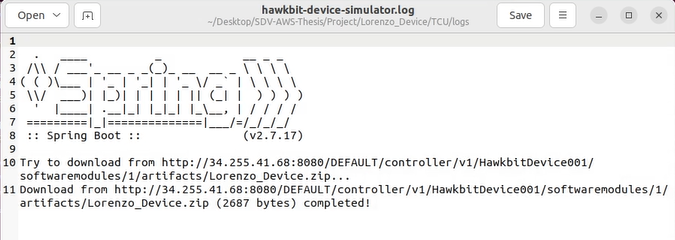
\includegraphics[width=0.8\textwidth]{images/update_log_HDS.png}  % Sostituisci 'nome_immagine' con il nome del tuo file immagine e l'estensione
    \caption{Update log file of the \textit{Device Simulator}}
    \label{fig:update_log_HDS}
\end{figure} 

The third component of the simulator is the heart of the \gls{ac:tcu}, which is the system that can generate the simulated vehicle data that changes in a progressive manner over time. This component has undergone several modifications during the course of development, in particular it was initially designed as a command line interface device written in \textit{Python} language.

More specifically, as shown in Figure \ref{fig:telemetryV1}, in the first version of the simulator, once started, based on commands given by the user via the command line, it was able to increase or decrease its simulated speed to a limit until it stopped. The speed information, which varied over time, was sent every second to the component that manages communication with the \textit{AWS IoT Core} server and then sent to the server.

\begin{figure}[h]  % 'h' significa che la figura viene posizionata qui
    \centering
    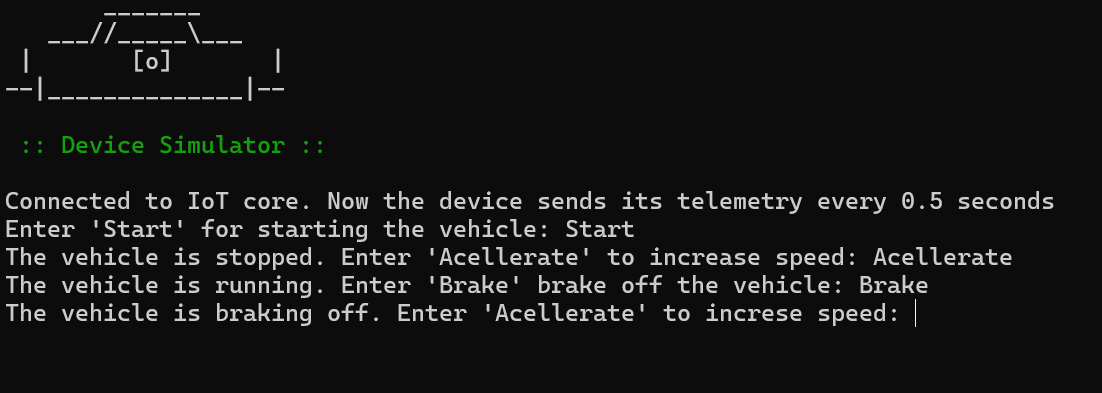
\includegraphics[width=0.8\textwidth]{images/telemetryV1.png}  % Sostituisci 'nome_immagine' con il nome del tuo file immagine e l'estensione
    \caption{A snapshot of the first version of the TCU interface}
    \label{fig:telemetryV1}
\end{figure} 

In this case, there were two different versions of the speed handler code: the first one represented the initial state of the simulated vehicle, while the second one represented the vehicle after the update. In this way, it was clear that the update of the vehicle had occurred.

At a later stage, for the creation of the final \textit{Python} \gls{ac:tcu}, it was decided to increase the number of telemetry data provided in such a way as to be able to collect and analyze a more realistic number of values in the cloud, but at the expense of a predefined data generation not decided by the user. This solution solved the fact that a real \gls{ac:tcu} would not present a graphical interface, but would simply collect the data generated by the subsystems present in the vehicle as a function of time. In this case, it was possible to build five subsystems capable of generating data every second in a way that can be considered as close as possible to a real system, then this data is collected by an orchestrating script \ref{lst:TCUOrchestrator} that aggregates it to make it ready to be sent to the listening cloud service.
\begin{lstlisting}[language=Python, caption={\gls{ac:tcu} orchestrator that collects data from other subsystems}, label=lst:TCUOrchestrator]
for sub in subsystems:
    values[sub.get_name()] = sub.get_info(t)
    values["Timestamp"] = datetime.isoformat(datetime.utcnow())
    values["DeviceID"] = f"{VIN}"
    print(values)
    messageFinal=json.dumps(values)
    mqttc.publish(publish_topic, messageFinal, 0)    
\end{lstlisting}

As shown in code \ref{lst:TCUOrchestrator}, an iteration is performed on each subsystem present in the simulator, the data is collected in \textit{Json} format and sent to the \textit{AWS IoT Core} service through the previously seen object in script \ref{lst:MQTTConnection} to establish the connection with the service itself. This system allows you to have maximum modularity of the subsystems, therefore possibly being able to add new ones with future updates, the only constraint is to specify the list of present subsystems in the \textit{Python} init \ref{lst:TCUInit} file and then add any new subsystems present.
\begin{lstlisting}[language=Python, caption={TCU init file for the import of the TCU subsystems}, label=lst:TCUInit]
from .airConditioning import AirConditioning
from .airbag import Airbag
from .heatedSeats import HeatedSeats
from .abs import ABS
from .engine import Engine
from .battery import Battery
subsystems = [Engine(), Battery(), AirConditioning(), Airbag(), HeatedSeats(), ABS()]  
\end{lstlisting}

Now, we will examine one of the sample subsystems developed for the project and assess its primary functions. A simulator has been implemented to generate data from a hypothetical vehicle battery in the case of hybrid or fully electric vehicles. This subsystem reports three main pieces of information: the energy added to the battery through regenerative braking, the total energy stored in the battery at a given moment, and the battery temperature at a given instant. The vehicle is considered a system where an electric motor provides energy during acceleration, causing a decrease in the battery's energy. During deceleration, part of the energy is stored in the battery through regenerative braking. The battery's temperature varies over time due to these operations.

The functions listed in code block \ref{lst:BatterySubsystem} are the most important parts of the class composing the subsystem simulator. These functions practically identify the common parts of each subsystem present in the project. The telemetry data is first aggregated in a \textit{Json} format and then returned by these functions. Additionally, a function is required to return an identifying name of the subsystem. This name is useful to the orchestrator shown previously in \ref{lst:TCUOrchestrator} at line 2 for constructing the data packet to be sent to the server correctly.
\begin{lstlisting}[language=Python, caption={Battery subsystem return code}, label=lst:BatterySubsystem]
def get_info(self, time):
    return {
        "StateOfCharge" : self.stateOfCharge,
        "BatteryTemperature": self.batteryTemperature,
        "EnergyAdded" : self.energyAdded,
    }
def get_name(self):
    return "Battery"  
\end{lstlisting}
During the updating phase, this data \ref{fig:TCUsimulatorP}, as well as all other subsystems, is created using a different algorithm. This ensures that when the telemetry data is analyzed, the download event is clearly visible. It is important to note that each \textit{Python} subsystem has a related set of tests that can be utilized by the cloud structure, as analyzed further below.
\begin{figure}[h]  % 'h' significa che la figura viene posizionata qui
    \centering
    \includegraphics[width=0.8\textwidth]{images/TCUsimulatorP.png}  % Sostituisci 'nome_immagine' con il nome del tuo file immagine e l'estensione
    \caption{A snapshot of the \gls{ac:tcu} simulator on the virtual machine}
    \label{fig:TCUsimulatorP}
\end{figure}

In the final phase of the project, it was decided to modify the simulator to use a compiled script. This change makes the system more similar to a real world situation, since in a real environment there would be systems where it is not possible to have scripts based on interpreters such as the \textit{Python} language, for reasons of size and resources, but where compiled programs are needed, which are more optimized. In order to do so and to give a concrete demonstration of the changes made to the infrastructure as analyzed in the following, it was decided to create a much simpler \gls{ac:tcu} simulator in \textit{C} language (\textit{C} simulator code). 
\begin{figure}[h]  % 'h' significa che la figura viene posizionata qui
    \centering
    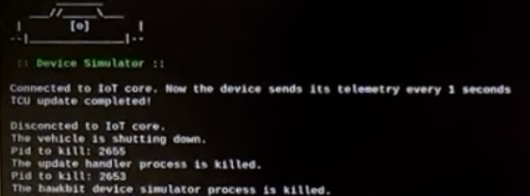
\includegraphics[width=0.8\textwidth]{images/TCUsimulatorC.png}  % Sostituisci 'nome_immagine' con il nome del tuo file immagine e l'estensione
    \caption{A snapshot of the \gls{ac:tcu} compiled simulator on the \textit{Raspberry Pi} interface}
    \label{fig:TCUsimulatorC}
\end{figure}

In order to be compatible with both the first and second versions of the simulator (for backward compatibility), it was also necessary to adapt the orchestrator element \ref{lst:TCUOrchestrator} to be capable of recognizing the type of simulator to which it would be interfaced with. To make this possible, a specification file indicating the type of simulator used \ref{lst:TCUManifest} was added to each \gls{ac:tcu} simulator.
\begin{lstlisting}[language=c, caption={Manifest example of compiled \gls{ac:tcu} simulator}, label=lst:TCUManifest]
<?xml version="1.0" encoding="UTF-8" standalone="yes"?>
<project>
    <name>C Project</name>
    <language>C</language>
    <compiler>gcc</compiler>
    <build_command>gcc main.c -o main.exe</build_command>
    <run_command>./main.exe</run_command>
</project>
\end{lstlisting}

The \gls{ac:tcu} simulator's download recognition system is the last element to be explored in detail. It is capable of activating downloads and ensuring that new elements are fully functional within the \gls{ac:tcu} system. Essentially, it functions as an edge agent, providing some of the tasks that the \textit{AWS IoT Greengrass} service would have performed in parallel if \textit{AWS IoT Greengrass} had been used on the edge device.
\begin{lstlisting}[language=Python, caption={Main function of the update recognition system }, label=lst:UpdateRecognition]
from watchdog.observers import Observer
from watchdog.events import FileSystemEventHandler
folder_to_watch = './TCU' # Define the folder to monitor
def main():
    global observer
    while True:
        observer = Observer() # Create an observer
        event_handler = DownloadHandler()
        observer.schedule(event_handler, folder_to_watch, recursive=True) # Attach the event handler to the observer
        observer.daemon = True
        observer.start() # Start the observer in a separate thread
        observer.join()  # Wait for the observer to finish operations

class DownloadHandler(FileSystemEventHandler):
    def on_created(self, event):
        update_file(event)
                        
    def on_modified(self, event):
        update_file(event)
\end{lstlisting}

The \textit{Python} script remains in an infinite loop, waiting for changes to the folder defined in line 3, using the libraries shown in lines 1 and 2 of code \ref{lst:UpdateRecognition}.
If a folder is created or modified, and updates from the server infrastructure are downloaded (which will be analyzed in a later subsection), this program aims to detect the processes involved in the execution of the \gls{ac:tcu} simulator (as done in lines 3 and 12 of code \ref{lst:UpdateFile}) and kill the identified processes. Meanwhile, the update file will be identified by a compressed folder, as specified by the update pipeline (which will be analyzed later). The update files will then be extracted according to line 19 of the code. Finally, this component will reboot the entire system so that the update can be installed and take effect.
\begin{lstlisting}[language=Python, caption={Code for performing actions when the designated download folder is changed}, label=lst:UpdateFile]
def update_file(event):
    global observer
    process = subprocess.Popen(["pgrep", "-f", "OS.py"], stdout=subprocess.PIPE, text=True)
    output, _ = process.communicate()
    pid_to_kill_list = output.splitlines()
    if not event.is_directory and ('downloads' in event.src_path): #If the new item is a directory
        print(f"src_path type: {type(event.src_path)}")
        print(f"New file downloaded: {event.src_path}")
        for pid_to_kill in pid_to_kill_list:
            print(f"Pid to kill: {pid_to_kill}")
            os.kill(int(pid_to_kill), signal.SIGTERM)    
        process = subprocess.Popen(["pgrep", "-f", "start.sh"], stdout=subprocess.PIPE, text=True)
        output, _ = process.communicate()
        pid_to_kill_list = output.splitlines()
        for pid_to_kill in pid_to_kill_list:
            print(f"Pid to kill: {pid_to_kill}")
            os.kill(int(pid_to_kill), signal.SIGTERM) #Kill the process
        if '.zip' in event.src_path:
            with zipfile.ZipFile(event.src_path, 'r') as zip_ref:
                zip_ref.extractall(folder_to_watch)
        else:
            shutil.copy(event.src_path, folder_to_watch)          
        print("File updated!")
        observer.stop()
\end{lstlisting}

\begin{figure}[h]  % 'h' significa che la figura viene posizionata qui
    \centering
    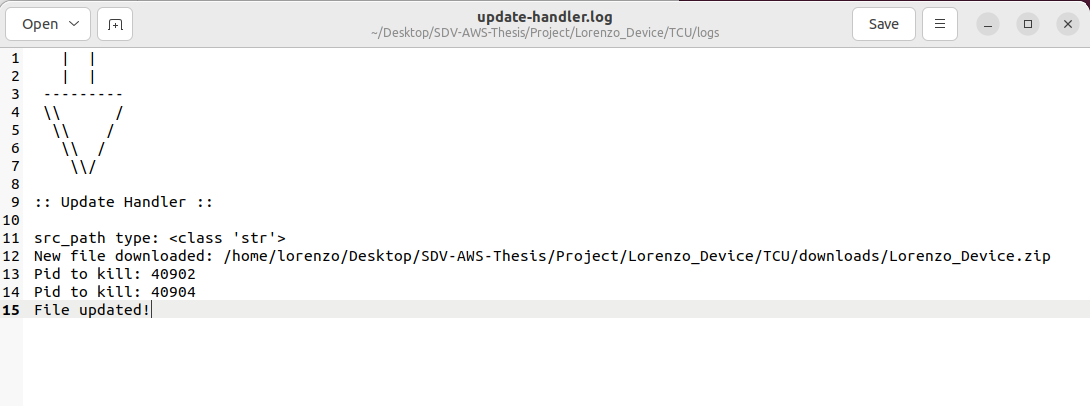
\includegraphics[width=0.8\textwidth]{images/watchdog_log.png}  % Sostituisci 'nome_immagine' con il nome del tuo file immagine e l'estensione
    \caption{A snapshot of the TCU recognition module logs}
    \label{fig:Watchdog_log}
\end{figure}

The \gls{ac:tcu} simulator is composed of the three elements analyzed so far, and their evolution during the project made it possible to create a system compatible with systems based on \textit{Arm} architectures, that is the \textit{Raspberry Pi}, capable of generating telemetry data and sending them to the cloud server connected through \textit{AWS IoT Core}, receiving updates, and rebooting the system to make the updates effective and active. Simulations were performed on virtual machines with "x86 architecture processors". The project will proceed to real test phases on actual systems once all necessary information has been acquired.

\subsection{Cloud Infrastructure}
Now the core of the project will be analyzed in detail, which is the cloud structure that allows, through the services offered by \gls{ac:aws} previously introduced, both the connection of the vehicle to send, analyze and manipulate data telemetry, and the cloud structure that allows the execution of the \textit{Hawkbit} server for the deployment of the update. This part of the project, as well as the previous one of the \gls{ac:tcu} simulator, experienced several changes during the implementation of the project, starting from a more experimental part of analysis and study of the various services, passing through a part of use more concretely linked to the development of the project, always relying on the console visualization tools, to arrive at a phase of creation of the entire structure through \gls{ac:cdk}, by executing the various stacks using \textit{Python} script. To avoid unnecessary repetition of operations, to simplify things, it was decided to directly analyze the structure of the stack built with \gls{ac:cdk}. In the following sections, each component of the structure will be examined in detail, assuming that there is already a general and theoretical knowledge of the various services used.

The initial stack analyzed is related to the construction of \textit{AWS IoT Core} services for device connectivity, that is, the connection of the \gls{ac:tcu} simulator to the cloud service for collecting telemetry data. In order to utilize the \textit{AWS IoT Core} service, an \textit{AWS IoT Core Thing} had to be defined, which can be described as the cloud-based version of the device's digital twin. After creating the \gls{ac:iot} device assigning it a name (as shown in line 1 of code \ref{lst:AWSIoTThing}), policies were added to enable connection with the \gls{ac:tcu} simulator and exchange of telemetry data via the \gls{ac:mqtt} protocol (line 4).
\begin{lstlisting}[language=Python, caption={Code for the creation of \textit{AWS IoT Core Thing} and related policies}, label=lst:AWSIoTThing]
cfn_thing=iot.CfnThing(self, "HawkbitDevice",
    thing_name="HawkbitDevice001"
)
cfn_policy = iot.CfnPolicy(self, "CfnPolicy", # Create a policy of the certificate
    policy_document={
    "Version":"2012-10-17",
    "Statement":[{
        "Effect":"Allow",
        "Action":["iot:Connect"],
        "Resource":[f"arn:aws:iot:"+region+":"+account+":client/" + cfn_thing.thing_name]
    },
    {
        "Effect": "Allow",
        "Action": ["iot:Publish"],
        "Resource":[f"arn:aws:iot:"+region+":"+account+":topic/*"]
    }]},
    policy_name=f"{cfn_thing.thing_name}IoTCertPolicy",
)
\end{lstlisting}
Note that, in this and all other stacks, the region and account \gls{ac:id} are taken directly from the \gls{ac:cdk} functionality.
The process of creating certificates was then implemented using \textit{Boto3} functions to save resources. Code \ref{lst:BotoIoTThingCert} certificates and their related keys are generated using a string seed and saved in a local directory for use in the physical device. The certificates are then returned to the \gls{ac:cdk} for use by the stack in saving to the \textit{AWS IoT Core Thing}. The two-second waiting period at line 23 is a precautionary measure to ensure the completion of the certificate creation operation.
\begin{lstlisting}[language=Python, caption={Code for the creation of \textit{AWS IoT Core Thing} certificates and keys}, label=lst:BotoIoTThingCert]
import boto3
import os
SECRET_NAME = "****"
iot = boto3.client('iot', region_name='*****')
def on_create(thing_name):
    response = iot.create_keys_and_certificate(setAsActive=True)
    certificate_id = response['certificateId']
    certificate_pem = response['certificatePem']
    key_pair = response['keyPair']
    directory_path="./certificates"
    if not os.path.exists(directory_path):
        os.makedirs(directory_path)
    file_path = os.path.join(directory_path, f"{thing_name}.private.key")
    with open(file_path, 'w') as file:
        file.write(key_pair['PrivateKey'])
    file_path = os.path.join(directory_path, f"{thing_name}.public.key")
    with open(file_path, 'w') as file:
        file.write(key_pair['PublicKey'])
    file_path = os.path.join(directory_path, f"{thing_name}.cert.pem")
    with open(file_path, 'w') as file:
        file.write(certificate_pem)
    time.sleep(2)
    return {
        'PhysicalResourceId': certificate_id,
        'Data': {
            'certificateId': certificate_id
    }}
\end{lstlisting}

To enable the creation of security files via \textit{Boto3}, separate from the \gls{ac:cdk} stack, a status variable was introduced to indicate the deploy or destroy status of the system \ref{lst:AWSIoTThingCert}. This was necessary to synchronize the deployment of the certificate and keys. Contrary to the rest of the mechanisms built into the \gls{ac:cdk}, the \textit{Boto3} functions are independent and not affected by the \gls{ac:cdk} commands. If this state variable had not been used, there would have been a misalignment between \gls{ac:cdk} stack for the \textit{AWS IoT Core Thing} creation and \textit{Boto3} certificates. \gls{ac:cdk} functions can be used to destroy the certificate and keys as in line 5. Finally, the created certificate is linked to the relevant policy and to the \textit{AWS IoT Core Thing} for proper usage.
\begin{lstlisting}[language=Python, caption={Code for the creation and destruction of \textit{AWS IoT Core Thing} certificates and keys from the \gls{ac:cdk} stack}, label=lst:AWSIoTThingCert]
if (status=="deploy"): # Creation of certificate with Boto3
    certificate=cert_handler(cfn_thing.thing_name)
else:
    certificate={"Data": {"certificateId": "Null"}}
print(f"{certificate['Data']['certificateId']}")
deactive_certificate_resource = cr.AwsCustomResource(self, "DeactiveCertificateResource",
    on_delete=cr.AwsSdkCall(
        service="Iot",
        action="UpdateCertificate",
        parameters={
            "certificateId": f"{certificate['Data']['certificateId']}",
            "newStatus": "INACTIVE",
    },),
    policy=cr.AwsCustomResourcePolicy.from_sdk_calls(
        resources=cr.AwsCustomResourcePolicy.ANY_RESOURCE
))
delete_certificate_resource = cr.AwsCustomResource(self, "DeleteCertificateResource", # Destruction of certificates
        service="Iot",
        action="DeleteCertificate",
        parameters={
            "certificateId": f"{certificate['Data']['certificateId']}",
            "forceDelete": f"{True}"
    },),
    policy=cr.AwsCustomResourcePolicy.from_sdk_calls(
        resources=cr.AwsCustomResourcePolicy.ANY_RESOURCE
))
deactive_certificate_resource.node.add_dependency( delete_certificate_resource )
\end{lstlisting}

The next step in building the cloud infrastructure involves creating the necessary environment for the \textit{Hawkbit} server. The idea is to use a basic \gls{ac:aec2} machine to build the server on, which, as discussed later, will be contacted by the \textit{AWS Codepipeline} via the server's \gls{ac:api} interfaces to deploy the updates. To create the \gls{ac:aec2} instance, as shown in code \ref{lst:AWSEC2Istance}, requires a \gls{ac:avpc} network in which to insert the instance itself as in line 1, an \gls{ac:ami} that contains everything necessary for the computer to run properly (line 2), and a role that can provide the correct policies for the computer to function properly (line 3).

\begin{lstlisting}[language=Python, caption={Code for the creation the \textit{EC2 Hawkbit} server istance}, label=lst:AWSEC2Istance]
vpc = ec2.Vpc(self, "VPC",
    nat_gateways=0,
    subnet_configuration=[ ec2.SubnetConfiguration( name="public",subnet_type=ec2.SubnetType.PUBLIC ) ]
)
generic_linux = ec2.MachineImage.generic_linux({  # AMI
    'eu-west-1': 'ami-0905a3c97561e0b69',
})
role = iam.Role(self, "InstanceSSM", assumed_by=iam.ServicePrincipal("ec2.amazonaws.com")) 
role.add_managed_policy( iam.ManagedPolicy.from_aws_managed_policy_name( "AmazonSSMManagedInstanceCore" ) )
instance = ec2.Instance(self, "Instance", # Instance
    instance_type=ec2.InstanceType("t2.small"),
    machine_image=generic_linux,
    vpc = vpc,
    role = role,
)
\end{lstlisting}

After creating the \gls{ac:aec2} machine instance, it is necessary to modify its properties to ensure correct operation of the \textit{Hawkbit} server. Specifically, two ports must be opened for \gls{ac:http} connections \ref{lst:AWSEC2Ports}. This allows the server to be accessible to both the \textit{CodePipeline} for deploying updates from the \textit{CodePipeline} to the server, and the \gls{ac:tcu} simulator device for downloading updates from the server to the edge device \cite{HawkbitDockerCompose}.
\begin{lstlisting}[language=Python, caption={Code for opening the doors}, label=lst:AWSEC2Ports]
instance.connections.connections.allow_from_any_ipv4( ec2.Port.tcp(8080), "Allow inbound HTTP traffic" )
instance.connections.connections.allow_from_any_ipv4( ec2.Port.tcp(5672), "Allow inbound HTTP traffic" )
\end{lstlisting}

At this step, it is possible to insert commands directly into the created machine, which are interpreted as command-line inputs necessary to start the server via the \textit{Docker} image \ref{lst:AWSEC2Commands}. Specifically, a \textit{Docker-compose} file is used to instantiate all the necessary server elements, including a database to record various information and a queue manager to manage external connections \ref{lst:AWSEC2DockerCompose}. Note that the properties mentioned in the code on line 36 are present in a local file. These properties are necessary to set the correct \gls{ac:ip} address in the server's \textit{Docker} image interface. The \textit{Docker-compose} file was created based on information from the \textit{Hawkbit} guide.
\begin{lstlisting}[language=Python, caption={Code to run commands on the machine}, label=lst:AWSEC2Commands]
file_path = "./files/docker-compose.yml"
with open(file_path, 'r') as file:
    docker_compose = file.read()
instance.user_data.add_commands(
    'sudo apt-get update -y',
    'sudo apt-get install -y docker-compose',
    f'sudo echo -e "{docker_compose}" > /home/ubuntu/docker-compose.yml',
    'sudo sed -i "s/\[server_ip_address\]/$(sudo curl -s http://169.254.169.254/latest/meta-data/public-ipv4)/g" /home/ubuntu/docker-compose.yml',
    'sudo docker-compose -f /home/ubuntu/docker-compose.yml up -d',
)
\end{lstlisting}

\begin{lstlisting}[language=Python, caption={\textit{Hawkbit} server \textit{Docker} compose}, label=lst:AWSEC2DockerCompose]
version: '3'
services:
    rabbitmq:
    image: 'rabbitmq:3-management'
    restart: always
    ports:
        - '15672:15672'
        - '5672:5672'
    labels:
        NAME: 'rabbitmq'
    mysql:
    image: 'mysql:8.0'
    environment:
        MYSQL_DATABASE: 'hawkbit'
        # MYSQL_USER: 'root' is created by default in the container for mysql 8.0+
        MYSQL_ALLOW_EMPTY_PASSWORD: 'true'
    restart: always
    ports:
        - '3306:3306'
    labels:
        NAME: 'mysql'
    hawkbit:
    image: 'hawkbit/hawkbit-update-server:latest-mysql'
    environment:
        - 'SPRING_DATASOURCE_URL= jdbc:mariadb://mysql:3306/hawkbit'
        - 'SPRING_RABBITMQ_HOST=rabbitmq'
        - 'SPRING_RABBITMQ_USERNAME=guest'
        - 'SPRING_RABBITMQ_PASSWORD=guest'
        - 'SPRING_DATASOURCE_USERNAME=root'
        - 'HAWKBIT_ARTIFACT_URL_PROTOCOLS_DOWNLOAD-HTTP_HOSTNAME= [server_ip_address]'
        - 'HAWKBIT_ARTIFACT_URL_PROTOCOLS_DOWNLOAD-HTTP_IP= [server_ip_address]'
    restart: always
    ports:
        - '8080:8080'
    volumes:
        - ./application.properties: /opt/hawkbit/application.properties
    labels:
        NAME: 'hawkbit'
    \end{lstlisting}

The final step in the \textit{Hawkbit} \gls{ac:aec2} server stack involves saving the necessary parameters in the \textit{Parameter Store} of the \textit{System Manager} to connect the \textit{AWS CodePipeline} with the \textit{Hawkbit} server via its \gls{ac:api}s. For example, let's consider the saving of one of the parameters, specifically the \gls{ac:ip} address of the \gls{ac:aec2} machine in code \ref{lst:AWSEC2ParameterStore}. The interaction with the \textit{System Manager} was performed using custom components of the \gls{ac:cdk}. The identifying name of the parameter, the value, and the type of the variable to be saved are indicated from line 5. In this case, the variable will simply be saved as a \textit{String} since it does not need to be obscured, this is different from the user's password, which is saved as \textit{SecureString}. The address is retrieved from the newly created instance using \gls{ac:cdk} functions in the line 7 of the code. The \textit{Lambda} functions utilized in the \textit{CodePipeline} will then access the saved parameters as will be examined later.
\begin{lstlisting}[language=Python, caption={Hawkbit server Docker compose}, label=lst:AWSEC2ParameterStore]
    create_param3 = cr.AwsCustomResource(self, "CreateParam3",
    on_create=cr.AwsSdkCall(
        service="SSM",
        action="PutParameter",
        parameters={
            "Name": "/hawkbitServer/ip_address",
            "Value": f"{instance.instance_public_ip}",
            "Type": "String"
        },
        physical_resource_id= cr.PhysicalResourceId.of("create_param3")
    ),
    on_delete=cr.AwsSdkCall(
        service="SSM",
        action="DeleteParameter",
        parameters={
            "Name": "/hawkbitServer/ip_address",
        },
        physical_resource_id= cr.PhysicalResourceId.of("delete_param3")
    ),
    policy=cr.AwsCustomResourcePolicy.from_sdk_calls(
        resources=cr.AwsCustomResourcePolicy.ANY_RESOURCE
))
\end{lstlisting}

Let's now analyze the construction of the pipeline for managing updates via \textit{\textit{CodePipeline}}. Two pipeline variants were elaborated during the development phase: one for managing updates via \textit{Python} scripts, and one for managing compiled updates, written in the \textit{C} language. To prevent description redundancy of the code, the two \textit{CodePipeline}s will be analyzed step by step. Common stages will be explained only once, while the specifics of the reference \textit{CodePipeline} will be discussed for the discordant parts. The \textit{Stack} for updates in \textit{C} language will serve as a reference for the common parts of \textit{CodePipeline}.
To begin, create a Codecommit repository for the pipeline source \ref{lst:AWSCodecommitRepo}. The \textit{CodeCommit} repository will contain the code and functionality to update the \gls{ac:tcu} simulator unit seen previously. The update will be created from a local \textit{ZIP} file as shown in line 4. For the C-compiled pipeline, use the source code provided in the zip file for compilation. The \textit{Python} script for the \textit{CodePipeline} \textit{Python} does not require compilation and will be ready to run in theory.
\begin{lstlisting}[language=Python, caption={CDK Code for the creation of the TCU simulator \textit{CodeCommit} repository}, label=lst:AWSCodecommitRepo]
code_repo = codecommit.Repository(
    self, "HawkbitDeviceC",
    repository_name="HawkbitDeviceC",
    code = codecommit.Code.from_zip_file( "./repos/Lorenzo_DeviceC.zip", "master" ) # Copies files from app directory to the repo as the initial commit
)
\end{lstlisting}

The \textit{CodeCommit} repository is placed in the first stage of the pipeline, as shown in \ref{lst:AWSCodecommitSource}. Each \textit{CodePipeline} stage can use an artifact as input and output. Since this is the first stage, only an output artifact is set, as shown in line 2. The pipelines require a default artifact bucket, which is an \gls{ac:as3} bucket or folder, as shown in line 1, and can be used by the pipeline if needed as will be shown in the actual pipeline creation phase later.
\begin{lstlisting}[language=Python, caption={CDK Code for the CodeCommit source stage set up}, label=lst:AWSCodecommitSource]
artifact_bucket = s3.Bucket.from_bucket_arn(self, f"codepipeline-{region}-****", f"arn:aws:s3:::codepipeline-{region}-****") #default codepipeline bucket
source_artifact = pipeline.Artifact("SourceArtifact")
source_stage = pipeline.StageProps(
    stage_name="Source",
    actions=[
        pipelineactions.CodeCommitSourceAction(
            action_name="CodeCommit",
            branch="master",
            output=source_artifact,
            repository=code_repo,
            variables_namespace="SourceVariables"
)])
\end{lstlisting}

The next stage requires separate and specific descriptions for both the \textit{Python} and \textit{C} pipelines. This stage concerns the build process. Specifically, for the build stage of the compiled update in \textit{C}, it is essential to establish a dedicated \textit{CodeBuild} stage for compiling \textit{C} scripts since it is not directly supported by the \textit{CodeBuild} service through the use of an \gls{ac:aecr} registry. A second supporting \textit{CodePipeline} is created by following the steps shown in code \ref{lst:AWSCPipeline}. The first step involves creating a \textit{CodeCommit} repository (at line 4) that contains the necessary information for building the new \textit{CodeBuild} module to compile the script. This includes a \textit{Dockerfile} for configuring the image with the necessary command to be created and a configuration file for the second pipeline build phase. The second stage of this pipeline involves the \textit{Codebuild} stage (line 20), which is the actual creation of the image, placed into a special \gls{ac:aecr} (line 15). This \gls{ac:aecr} is then used in the update pipeline. It is important to note that during the creation of the second pipeline different roles are created with the related policies for the interaction between the different components.
\begin{lstlisting}[language=Python, caption={CDK Code for the Codepipeline for the C compiled file build creation}, label=lst:AWSCPipeline]
C_custom_code_repo = codecommit.Repository(
    self, "HawkbitCCustomBuildImageRepo",
    repository_name="HawkbitCCustomBuildImage",
    code= codecommit.Code.from_zip_file( "./repos/HawkbitCCustomBuildImage.zip", "main" )
)
source_stage_c = pipeline.StageProps(
    stage_name="Source",
    actions=[
        pipelineactions.CodeCommitSourceAction(
            action_name="CodeCommit",
            branch="main",
            output=source_artifact_c,
            repository=C_custom_code_repo,
    )])
ecr_repository = ecr.Repository(self, "HawkbitCBlogRepo",
    repository_name="hawkbit-C-blog",
    removal_policy=RemovalPolicy.DESTROY,
    auto_delete_images=True,
)
C_custom_build = codebuild.Project(
    self, "HawkbitCCustomBuildImageBuild",
    build_spec=codebuild.BuildSpec.from_source_filename(
        "buildspec.yml"),
    source=codebuild.Source.code_commit(
        repository=C_custom_code_repo,
        branch_or_ref="master"),
    environment=codebuild.BuildEnvironment(
        build_image= codebuild.LinuxBuildImage.AMAZON_LINUX_2_ARM_2,
        privileged=True),
    role=codebuild_role,
    project_name="HawkbitCCustomBuildImage",
    environment_variables={
        'ecr': codebuild.BuildEnvironmentVariable(
            value=ecr_repository.repository_uri),
        'tag': codebuild.BuildEnvironmentVariable(
            value='v1'),
    },
    timeout=Duration.minutes(60)
)
C_custom_pipeline = pipeline.Pipeline(
    self, "hawkbit-device-c",
    pipeline_name="hawkbit-device-c",
    artifact_bucket=artifact_bucket,
    stages=[source_stage_c, build_stage_c]
)
\end{lstlisting}

In the initial \textit{CodePipeline}, a machine is built during the stage to compile the \textit{C} script from the source stage using the image saved in the previously analyzed \gls{ac:aecr}. At this point, the build stage can compile and build the necessary \textit{C} script for the update. The final result of this stage \ref{lst:AWSCodepipelineBuild} is an executable in the pipeline that contains the functionality produced by the \textit{C} script in the Source stage.
\begin{lstlisting}[language=Python, caption={CDK Code for the Codecommit build stage set up}, label=lst:AWSCodepipelineBuild]
hawkbit_build = codebuild.Project(
    self, "HawkbitDeviceBuildC",
    build_spec=codebuild.BuildSpec.from_source_filename(
        "buildspec.yml"),
    source=codebuild.Source.code_commit(
        repository=code_repo,
        branch_or_ref="master"
    ),
    environment=codebuild.BuildEnvironment(
        privileged=True,
        build_image= codebuild.LinuxArmBuildImage.from_ecr_repository( ecr_repository, "v1")
    ),
    project_name="HawkbitDeviceBuildC"
)

build_stage = pipeline.StageProps(
    stage_name="Build",
    actions=[
        pipelineactions.CodeBuildAction(
            action_name="Build",
            input=pipeline.Artifact("SourceArtifact"),
            project=hawkbit_build,
            outputs=[build_artifact]
    )])
\end{lstlisting}
\begin{figure}[h]  % 'h' significa che la figura viene posizionata qui
    \centering
    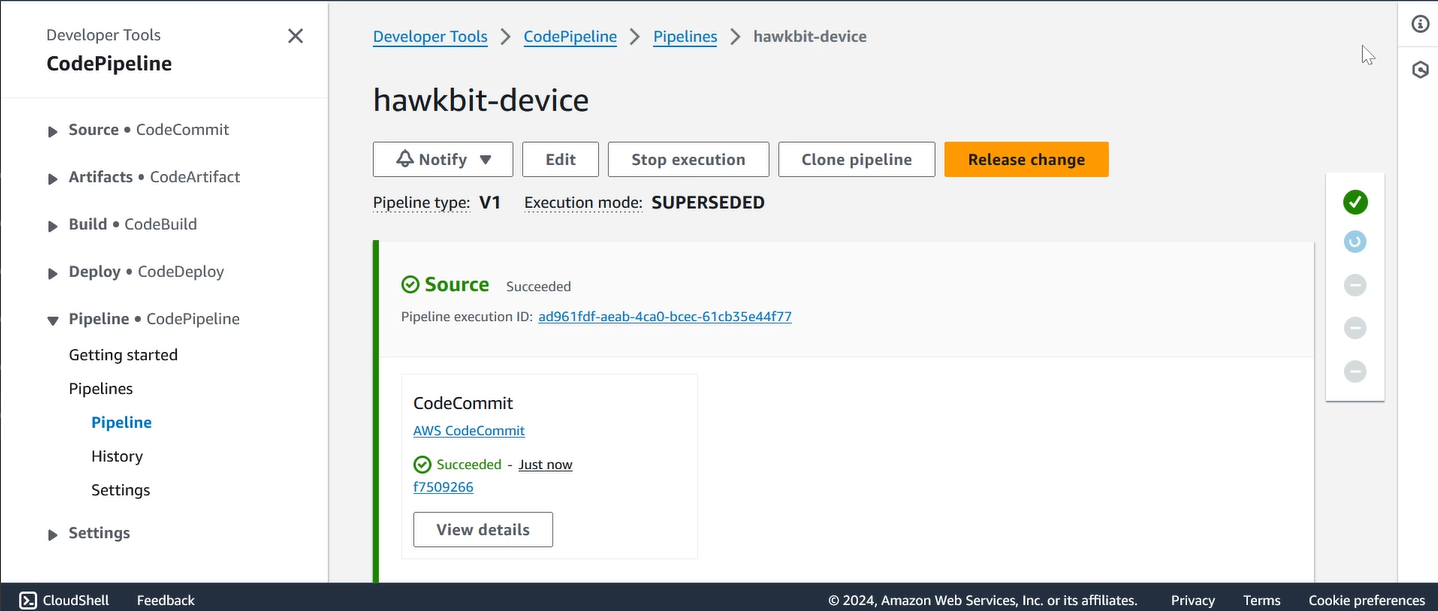
\includegraphics[width=0.8\textwidth]{images/hawkbitCodepipeline.png}  % Sostituisci 'nome_immagine' con il nome del tuo file immagine e l'estensione
    \caption{A snapshot of the Codepipeline Source stage}
    \label{fig:HawkbitCodepipeline}
\end{figure}

Regarding the \textit{Python} pipeline, the build stage is utilized as a test stage to launch tests built specifically for the repository code. This is due to the fact that \textit{Python} scripts do not require actual code compilation. Using the pytest tool, it is possible to initiate the battery of tests present in the code repository. This information is located in the build configuration file within the repository.

The next stage of both pipelines contains \textit{Lambda} functions that interact with the \textit{Hawkbit} server through its \gls{ac:api}. To ensure greater modularity, there are three \textit{Lambda} functions distributed over three different stages. As a first step, a dedicated role is created for each \textit{Lambda} function. This role contains the necessary policies for the function to perform its tasks once associated with the \textit{Lambda}.
Starting from the deployment stage of the software update on the \textit{Hawkbit} server, it is evident in code \ref{lst:AWSCodepipelineLambda} that the function is extracted from a local \textit{ZIP} file and uploaded to the \textit{Lambda} service, and this approach is followed for all subsequent \textit{Lambda} stages.
\begin{lstlisting}[language=Python, caption={CDK Code for the deploy software on Hawkbit server Lambda creation}, label=lst:AWSCodepipelineLambda]
lambda_function = _lambda.Function(
    self,"hawkbitDeploySoftwareOnHawkbitServer",
    function_name="hawkbitDeploySoftwareOnHawkbitServer",
    runtime=_lambda.Runtime.PYTHON_3_11,
    code=_lambda.Code.from_asset( "./lambda/hawkbitDeploySoftwareOnHawkbitServer.zip"),
    handler="hawkbitDeploySoftwareOnHawkbitServer.lambda_handler",
    role=lambda_role,
    log_retention=logs.RetentionDays.ONE_DAY,
    timeout=Duration.seconds(60)
)
hawkbitDeploySoftwareOnHawkbitServer_stage = pipeline.StageProps(
    stage_name="hawkbitDeploySoftwareOnHawkbitServer",
    actions=[hawkbitDeploySoftwareOnHawkbitServer_invoke],
)
\end{lstlisting}

When analyzing the Lambda function, it can be seen that the calls to the \textit{Hawkbit Server \gls{ac:api}}, after obtaining all the parameters necessary for execution, basically follow a fairly precise pattern. This is demonstrated in code \ref{lst:AWSLambdaSoftwareModule} for building the software module, which is the component of the \textit{Hawkbit} server that contains the update file. It starts by specifying the \gls{ac:url} of the server, then specifies the information to send in the request payload, then specifies the headers containing the authentication information, and finally sends the \gls{ac:http} request.
\begin{lstlisting}[language=Python, caption={Lambda code for the software module creation}, label=lst:AWSLambdaSoftwareModule]
url = f"http://{server_ip}:8080/rest/v1/softwaremodules"
payload = json.dumps([{
    "name": project_name,
    "version": project_version,
    "type": "Application",
    "description": "Hawkbit device simulator module from codecommit",
    "vendor": "Reply",
    "encrypted": False
}])
headers = {
    'Content-Type': 'application/json',
    'Authorization': auth_header
}
response = requests.request("POST", url, headers=headers, data=payload)
if response.status_code != 201:
    print(f"Error in the Software Module creation!  Error: {response.status_code}")
    traceback.print_exc()
    put_job_failure(job_id, 'Function exception: ')
    return
print('Software Module creation completed')
\end{lstlisting}

After creating the software module, the update file is retrieved from the \gls{ac:as3} bucket where it was saved in the source stage and loaded into the module. Then the distribution set is created following the same pattern as the previous software module. In this experimental project, the distribution set only contains one software module. It is important to note that any errors in these steps, like in any \textit{Lambda} stage, will cause the pipeline to abort and report the error.

After analyzing the \textit{Lambda} stage, the \textit{Hawkbit} server now has a distribution set that includes a software module. This module contains the update file that needs to be downloaded to the \gls{ac:tcu} simulator device. The \textit{CodePipeline} proceeds by creating two \textit{Lambda} stages that perform similar operations: deploying the distribution set to the device connected to the \gls{ac:ota} server. Specifically, in the first case reported in the code \ref{lst:AWSLambdaRollout} a roll-out is performed, creating a fleet of devices to which the update is scheduled. The pool of devices on which to roll out the update is selected by reviewing the devices currently connected to the \gls{ac:ota} server, so given the nature of the project, the pool will consist of only one edge device. In the second case, however, the update is directly assigned to the device. Both stages essentially perform the same operation, but they use different \gls{ac:api}s of the \textit{Hawkbit} server. Executing one stage excludes the execution of the other. The stages are designed to provide the user with the maximum \gls{ac:api} usability. 
\begin{lstlisting}[language=Python, caption={Lambda code for the roll out creation and execution}, label=lst:AWSLambdaRollout]
url = f"http://{server_ip}:8080/rest/v1/rollouts"
payload = json.dumps({
    "createdBy": "Reply",
    "createdAt": int(datetime.now().timestamp()),
    "lastModifiedBy": "Reply",
    "lastModifiedAt": int(datetime.now().timestamp()),
    "name": f"{distribution_set['name']}{distribution_set['version']}",
    "description": "Rollout on HawkbitDevice",
    "targetFilterQuery": f"id=={target_names}*",
    "distributionSetId": distribution_set['id'],
    "amountGroups": 1,
    "type": "forced"
})
headers = {
    'Content-Type': 'application/json',
    'Authorization': auth_header
}
response = requests.request("POST", url, headers=headers, data=payload)
url = f"http://{server_ip}:8080/rest/v1/rollouts/{rollout_id}/start"
payload = ""
headers = {
    'Content-Type': 'application/json',
    'Authorization': auth_header
}
response = requests.request("POST", url, headers=headers, data=payload)
\end{lstlisting}

As a last point in both analyzed \gls{ac:cdk} implementations the pipeline is declared with all the necessary stages so that it is built correctly. In practice with these stages it is possible to build or a test the source code as needed, and perform a deployment of the updates directly to the \gls{ac:tcu} simulator device through the use of the \textit{Hawkbit} server and its exposed \gls{ac:api}.
\begin{figure}[h]  % 'h' significa che la figura viene posizionata qui
    \centering
    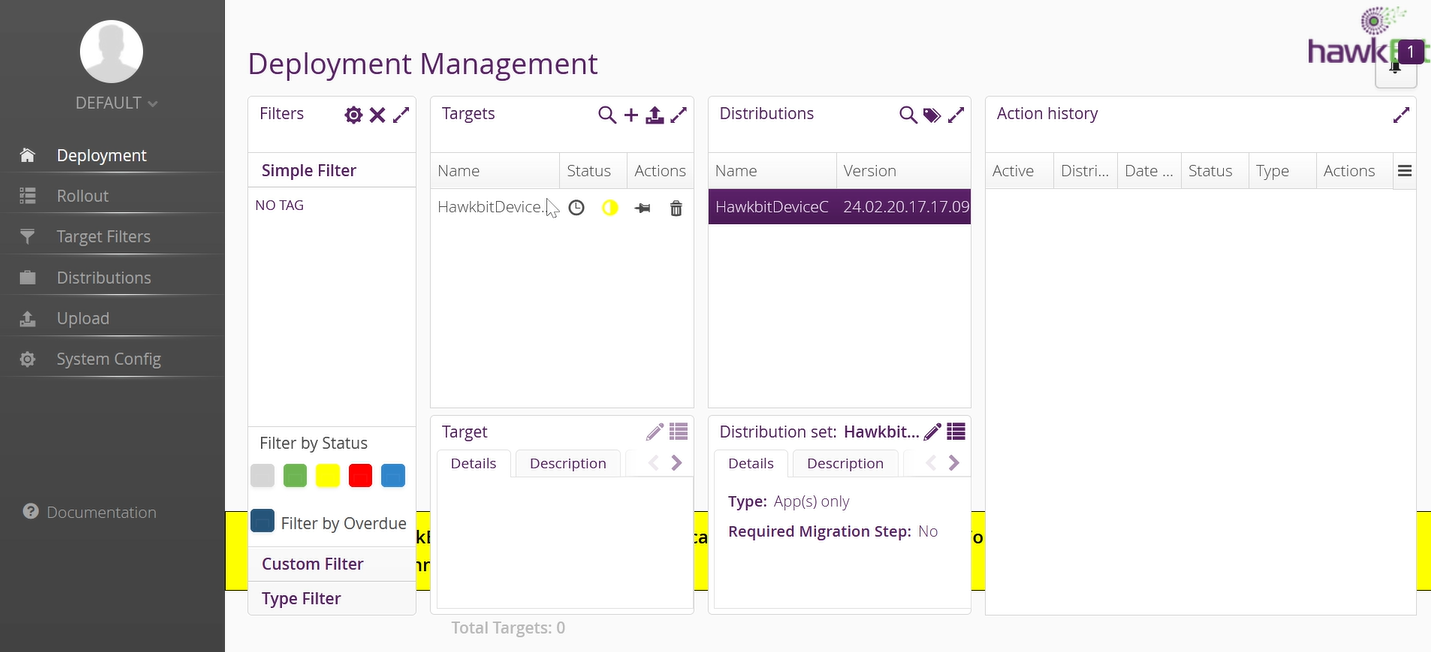
\includegraphics[width=0.8\textwidth]{images/hawkbit_server.png}  % Sostituisci 'nome_immagine' con il nome del tuo file immagine e l'estensione
    \caption{A snapshot of the Hawkbit server during the deployment of the update on the device}
    \label{fig:HawkbitServer}
\end{figure}
The final stack of the cloud infrastructure created by \gls{ac:cdk} is the actual data collection stack via \textit{AWS Timestream}. In this stack, a \textit{Kinesis Data Stream} is first created. The stream takes the data published to the channel created by the device via an \gls{ac:sql} query and routes it to a new destination. Next, the database and tables needed to store the telemetry data are created. Then, the \textit{Kinesis} stream is used as input, triggering the start of a \textit{Lambda} function that takes the output data from the stream as input, decompresses and formats it so that it can be handled by \textit{Timestream}, and finally sends it to the corresponding tables, which at this point already exist because they were created previously.
Upon analyzing code \ref{lst:AWSKinesis} in detail, it becomes clear that once the Kinesis Stram has been created, it is assigned a role for reading data from the channel (line 1) and then, via a rule to be executed, is given the very instruction to read data from the channel (line 14).
\begin{lstlisting}[language=Python, caption={CDK code for the creation of the Kinesis stream with its role and rule}, label=lst:AWSKinesis]
kinesis_stream = kinesis.Stream(self, "hawkbitDeviceData",
    stream_mode=kinesis.StreamMode.ON_DEMAND,
    stream_name="hawkbitDeviceData"
)
device_to_kinesis_role = iam.Role(self, "hawkbitDeviceToKinesis", assumed_by=iam.ServicePrincipal("iot.amazonaws.com"),  role_name="hawkbitDeviceToKinesis")
device_to_kinesis_role.add_to_policy(iam.PolicyStatement(
    effect=iam.Effect.ALLOW,
    actions=["kinesis:*"],
    resources=[kinesis_stream.stream_arn],
))
device_to_kinesis_rule = iot.CfnTopicRule(self, "fromDeviceToKinesis",
    rule_name="HawkbitDeviceDataToKinesis",
    topic_rule_payload=iot.CfnTopicRule.TopicRulePayloadProperty(
        sql="SELECT * FROM 'device/HawkbitDevice001/telemetry'",
        actions=[iot.CfnTopicRule.ActionProperty(
            kinesis=iot.CfnTopicRule.KinesisActionProperty(
                role_arn=device_to_kinesis_role.role_arn,
                stream_name=kinesis_stream.stream_name,
                partition_key="${DeviceID}"
),)]))
\end{lstlisting}
After creating the stream, the database is established. First, the general configuration settings are provided, including the data retention period and the identifying name. Then, the necessary tables shown in example code \ref{lst:AWSTimestreamTable} are created one by one. In this case, there are 5 tables since the \gls{ac:tcu} simulator device has 5 subsystems.
\begin{lstlisting}[language=Python, caption={CDK code for the creation of the Battery table of the Timestream database}, label=lst:AWSTimestreamTable]
Battery_table = timestream.CfnTable(self, "Battery", database_name=database.database_name,
    schema=timestream.CfnTable.SchemaProperty(
        composite_partition_key= [timestream.CfnTable.PartitionKeyProperty(
            type="DIMENSION",
            enforcement_in_record="REQUIRED",
            name="DeviceID"
    )]),
    retention_properties=retention,
    table_name="Battery",
)
Battery_table.add_dependency(database)
\end{lstlisting}
The \textit{Lambda} function is created at the end, with its policies attached to the role that was specifically created for it. As demonstrated in code \ref{lst:AWSTimestreamlambda}, the \textit{Lambda} is retrieved from a local file and imported into the \gls{ac:aws} service. In this case, the \textit{Lambda} function processes the received data by formatting the \textit{Json} format into a flat one, so that there are no table sub-levels because they are not supported by the \textit{Timestream} service, and organizes the data into the appropriate tables by making an association between the data name and the table name.
\begin{lstlisting}[language=Python, caption={CDK code for the creation of Lambda function that takes data from Kinesis stream and sends it to the Timestream tables}, label=lst:AWSTimestreamlambda]
lambda_function = _lambda.Function(
    self,"hawkbitFromKinesisToTimestream",
    function_name="hawkbitFromKinesisToTimestream",
    runtime=_lambda.Runtime.PYTHON_3_11,
    code=_lambda.Code.from_asset( "./lambda/hawkbitFromKinesisToTimestream.zip"),
    handler="hawkbitFromKinesisToTimestream.lambda_handler",
    role=lambda_role,
    timeout=Duration.seconds(60),
)
lambda_function.add_event_source(eventSources.KinesisEventSource(
    kinesis_stream,
    batch_size=100,  # default
    starting_position=_lambda.StartingPosition.LATEST
))
\end{lstlisting}
Now that the entire cloud infrastructure system has been established, it is possible to gain a better understanding of the interactions between its various components. The system begins with four basic elements: the \textit{IoT Core Thing}, the \textit{CodePipeline} pipeline, the \textit{Hawkbit} server, and the \textit{Timestrem} database. After creating the \textit{IoT Core} device, it can retrieve data that will be stored in the \textit{Timestrem} database. Updates can be deployed to the physical \gls{ac:tcu} simulator device through the Codepipeline pipeline and the \textit{Hawkbit} server. After installation, the data received by \textit{IoT Core} and stored in the database will undergo a change that can be detected during analysis. The process can be repeated indefinitely for any updates made to the code in the development repository.

\subsection{Data Viewer: Grafana}
\textit{Grafana} was selected to visualize the data in the \textit{Timestream} database. It natively supports linking to \textit{Timestream} service as a data source by providing account credentials. To use \textit{Grafana}, start a \textit{Docker} container containing the server to construct graphs using data from the chosen source, in this case, the \textit{Timestream} project.

To utilize the \textit{Grafana} server, a separate virtual machine was created to connect to the \textit{Timestream} database using \gls{ac:aws} credentials and retrieve the stored data. By querying the \textit{Timestream} tables, real-time graphs can be generated as the database is continuously updated. It is important to maintain a consistent update cadence between the \textit{Timestream} database and the \textit{Grafana} server. These queries produce a dataset that is plotted and interpreted differently depending on the type of graph used.

Real dashboards can be created by combining multiple graphs, even if they display the same data, to provide different perspectives. For the purposes of this project, it was decided to create three dashboards for three different taballe to represent data from the three most relevant subsystems of the \gls{ac:tcu} simulator. 

With the use of these dashboards as shown in Figure \ref{fig:GrafanaABS}, it was possible to clearly represent the successful update of the TCU simulator device. For instance, this example shows the simulation of a vehicle's battery system. The dashboard displays two progressive data sets over time and one instantaneous data set. Specifically, the bottom left corner of the dashboard shows the battery temperature over time. From this information, it is evident that the temperature exhibits greater oscillations following the update, while remaining around a precise value. The total amount of energy present in the battery is also displayed at the bottom right, although it is not possible to detect the presence of the update due to the instantaneous nature of the data. Above, the graph shows the progression of energy added to the battery over time. It is evident that after the update, the addition of energy to the battery increased significantly after one second. This observation is based on the detected data. With this update, the goal is basically to simulate an improvement in performance related to the recovery of energy from regenerative braking, and this is shown in the graph both with the fact that after a certain moment the energy present in the battery is higher, and with the fact that the total net energy accumulated by regenerative braking is higher after the update.
\begin{figure}[h]  % 'h' significa che la figura viene posizionata qui
    \centering
    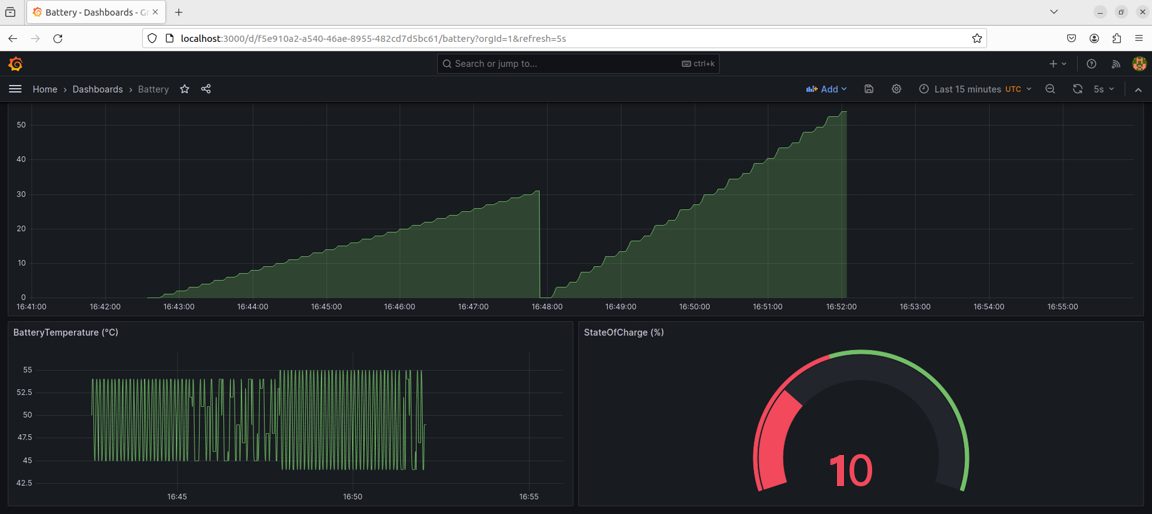
\includegraphics[width=0.8\textwidth]{images/grafana_Battery.png}  % Sostituisci 'nome_immagine' con il nome del tuo file immagine e l'estensione
    \caption{A snapshot of the ABS graph on the Grafana server}
    \label{fig:GrafanaABS}
\end{figure}

The dashboards for the \gls{ac:abs} system of the \gls{ac:tcu} simulator are produced in \textit{Graphana}. This allows for easy detection of updates through changes in the data. The data shows improved performance of regenerative braking, resulting in less energy needed for the physical brakes to apply to the discs. As a result, the simulated temperatures are lower. The dashboard for the vehicle's acceleration system is presented last.

To provide a complete summary of all the \gls{ac:poc} elements, the system interacts as described below. Firstly, launch the \gls{ac:cdk} script to activate the supporting cloud infrastructure immediately. This will also generate the necessary certificates for device authentication. Secondly, after correctly positioning the certificates, it will be necessary to start the \gls{ac:tcu} simulator device by providing the correct \gls{ac:ip} address of the \textit{Hawkbit} server to connect to for any future updates. Once a sufficient amount of data has been produced and analyzed in the \textit{Grafafana} dashboard, updates can be made. The \textit{AWS CodeCommit} repository can be used to produce a specific code that represents the source of the update. After a commit is made on the master branch, the pipeline will deploy the update on the \textit{Hawkbit} server and the device. Once the update is received, the \gls{ac:tcu} simulator will position the functions correctly and restart the system for the update to work effectively. At this point, there are two ways to evaluate the update: either through the log files produced directly on the device (if access to the physical device is available), or by analyzing the data produced by the \gls{ac:tcu} simulator after the update, which at this point will be different from the initial data. The execution of this complex system was confirmed during the testing phase with the demo on the real \textit{Raspberry Pi} device, as will be seen later.